\subsection{Overview: high-level components and their interaction}


\begin{figure} [!h]
	\centering
	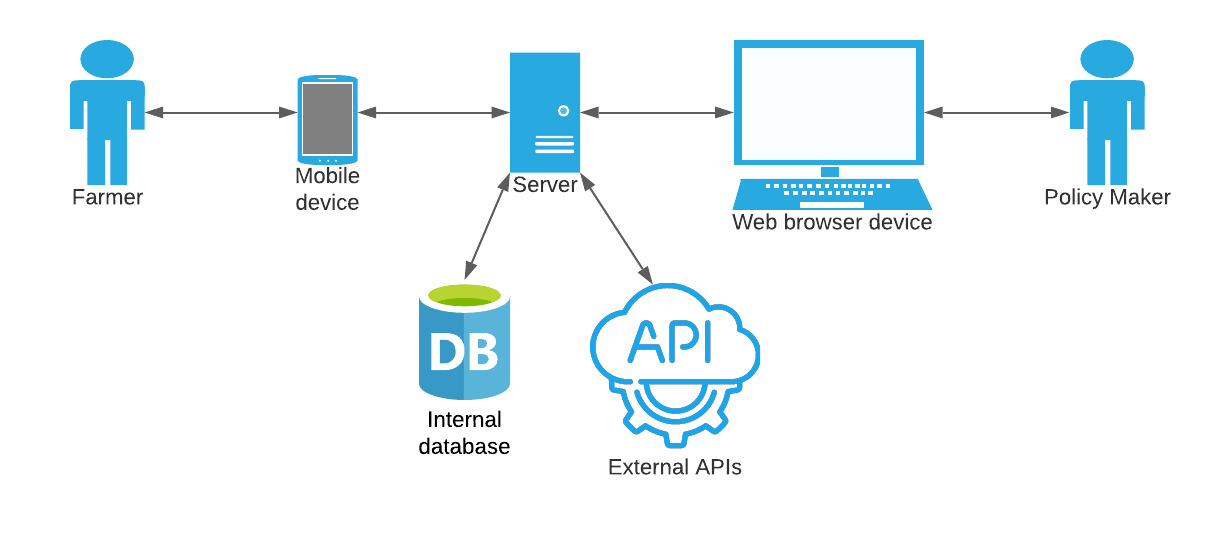
\includegraphics[width=\textwidth]{Images/architecture-diagram.png}
	\caption{\label{fig:physical_diag} Physical architecture diagram}
\end{figure}


\subsection{Component view}
\begin{figure} [!h]
	\centering
	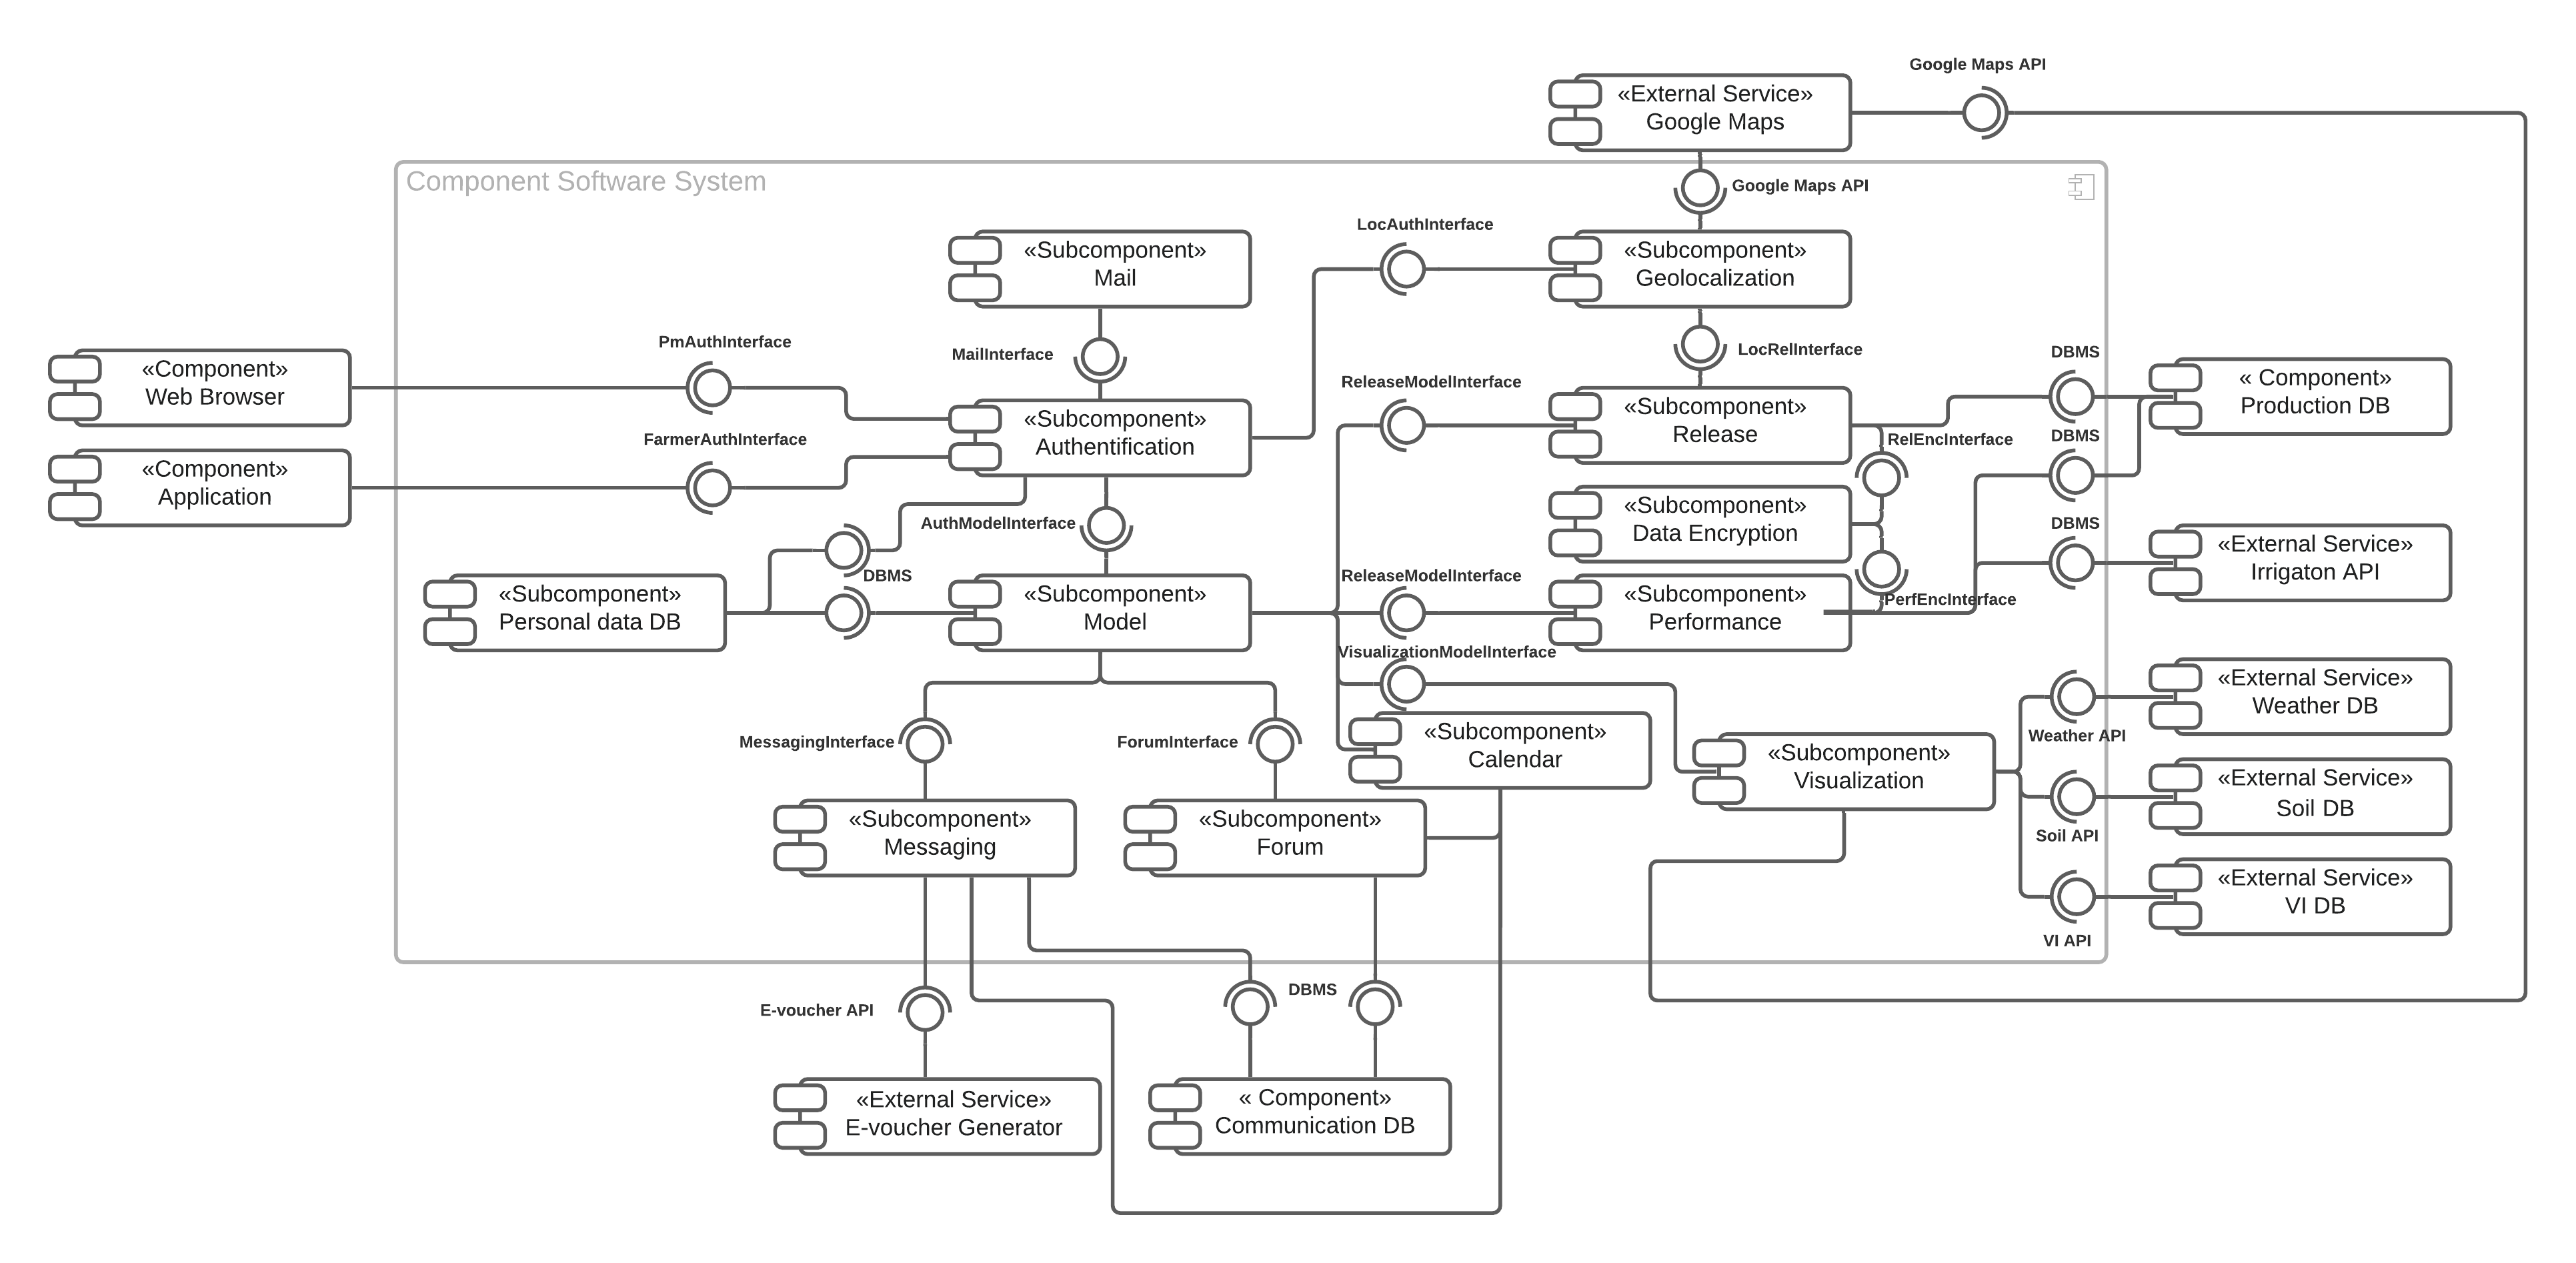
\includegraphics[width=\textwidth]{Images/component-diagram.png}
	\caption{\label{fig:component_diag} Component diagram}
\end{figure}

\subsection{Deployment view}
\begin{figure} [H]
	\centering
	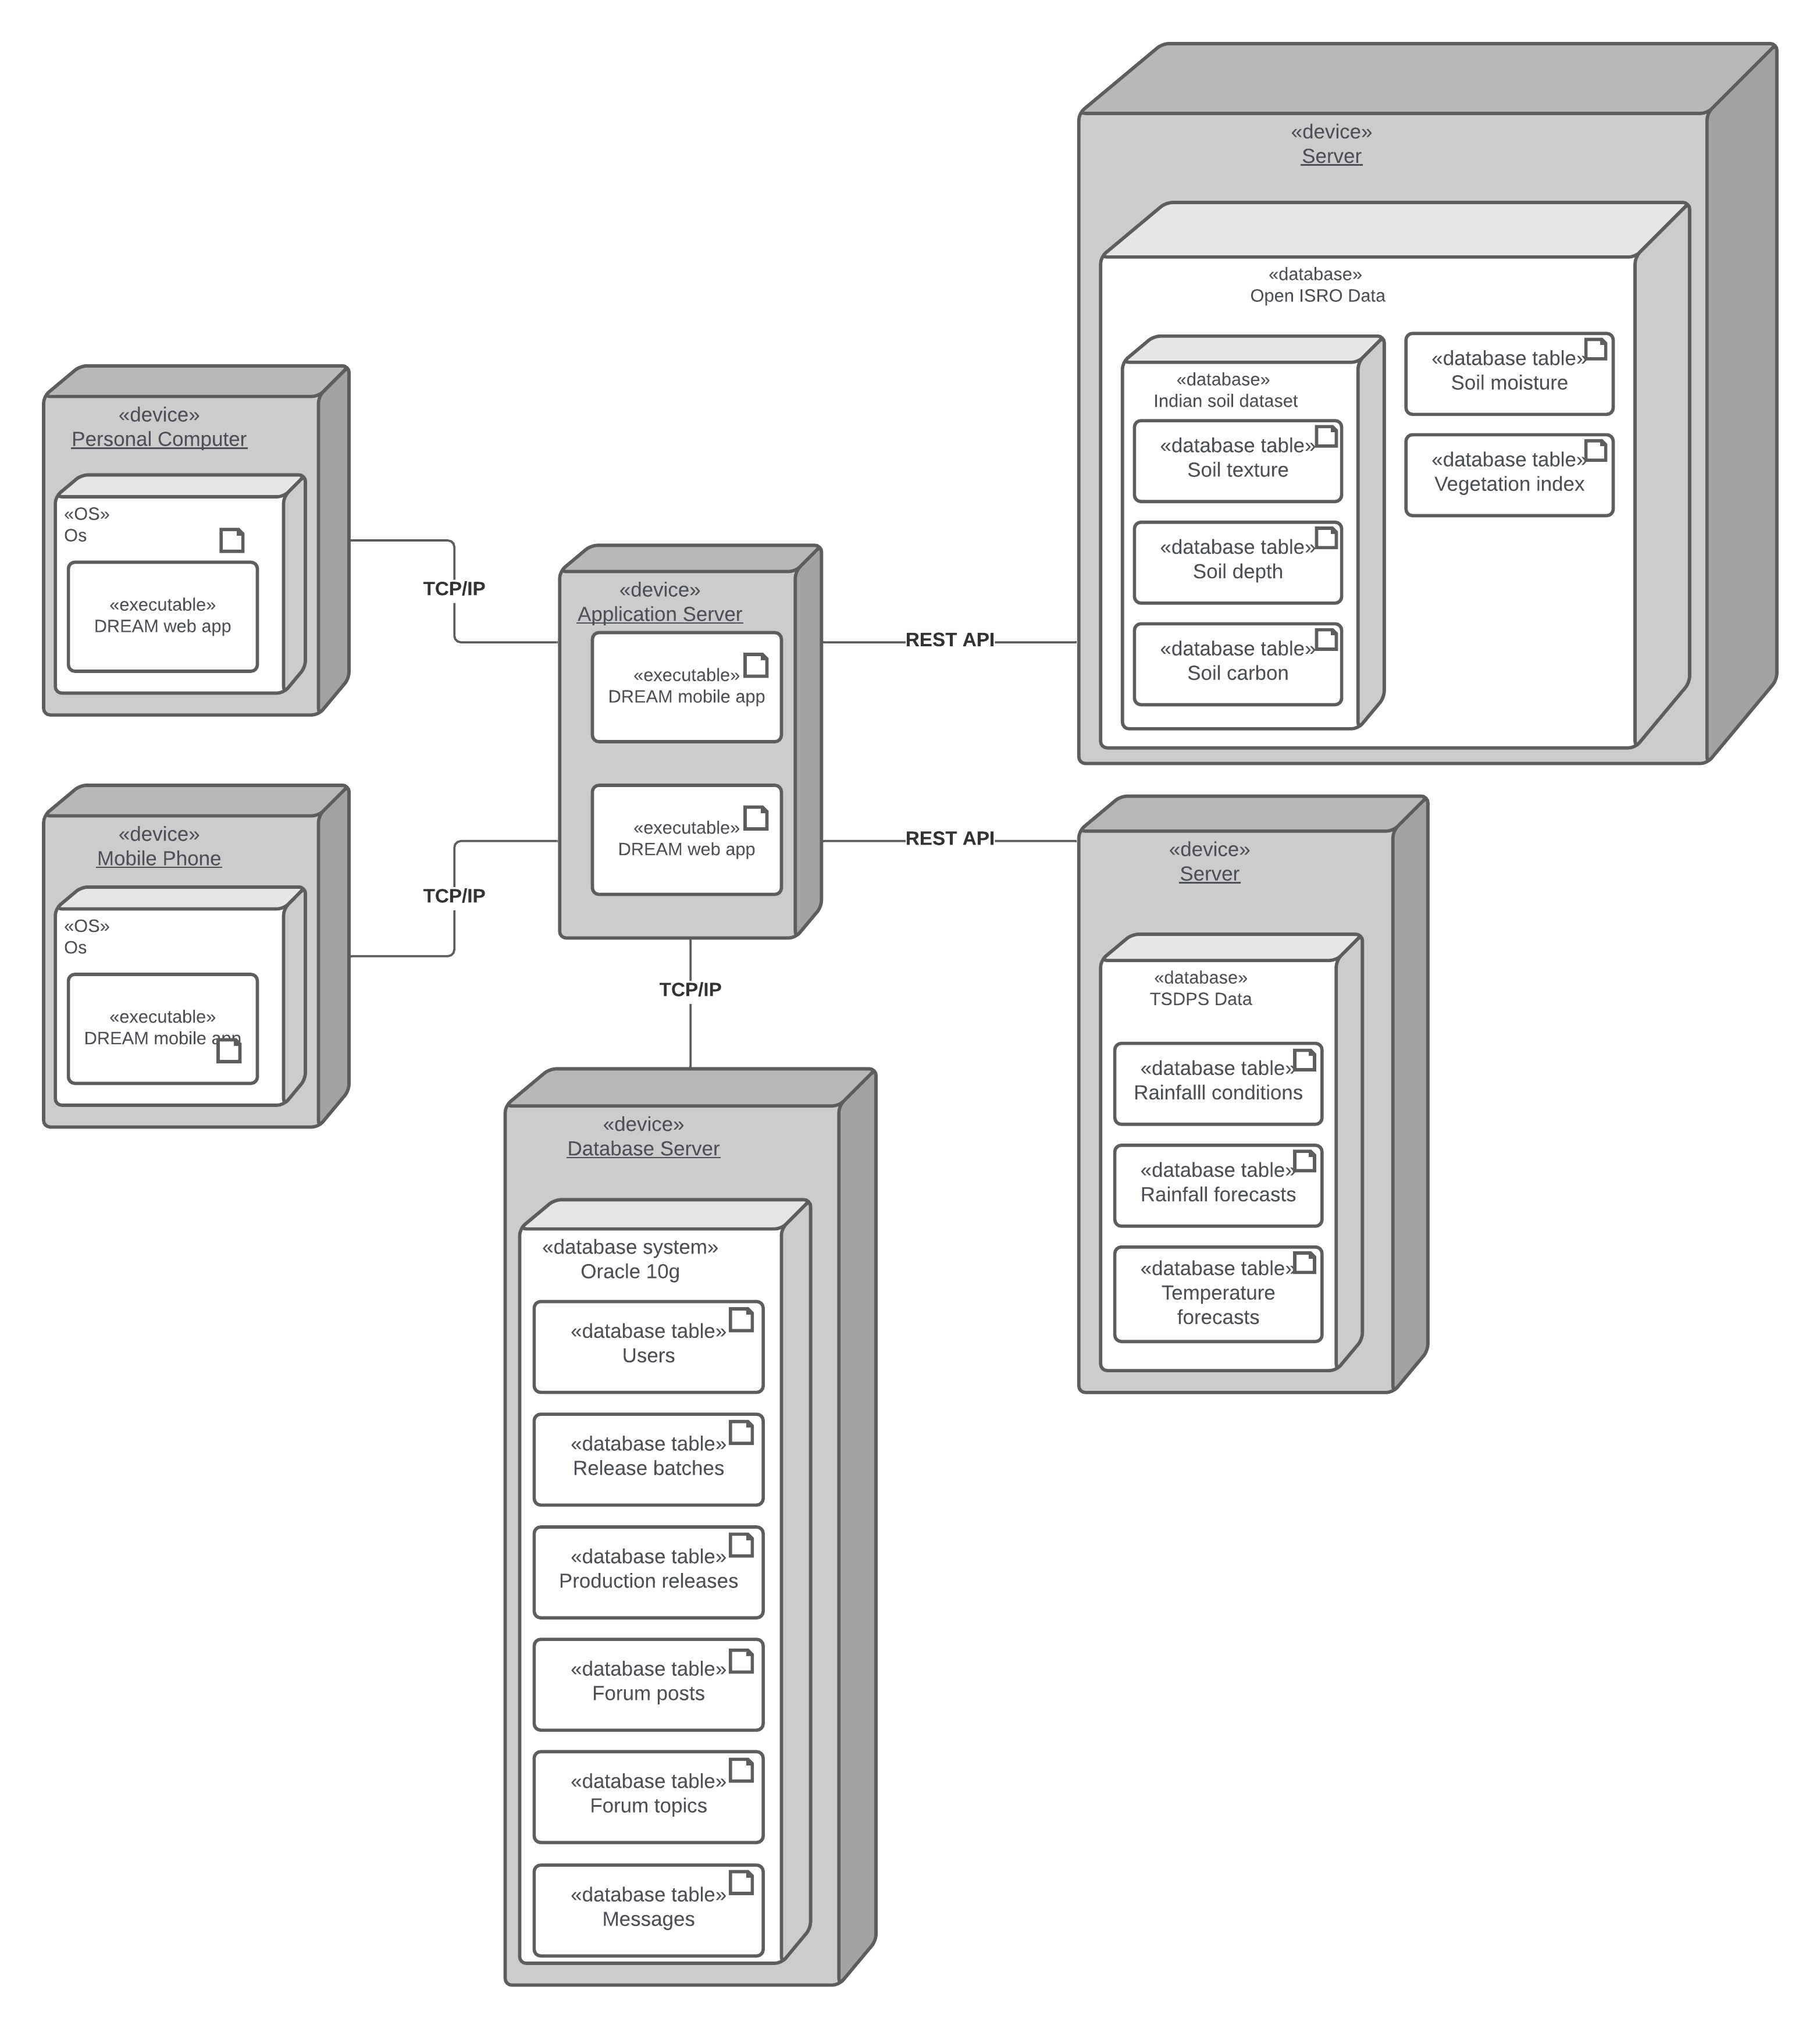
\includegraphics[width=\textwidth]{Images/deployment-view.png}
	\caption{\label{fig:component_diag} Deployment diagram}
\end{figure}

\subsection{Runtime view}
The following sequence diagrams aims at presenting the links between the component during the principal uses of the System by the different users.

\begin{figure} [H]
	\centering
	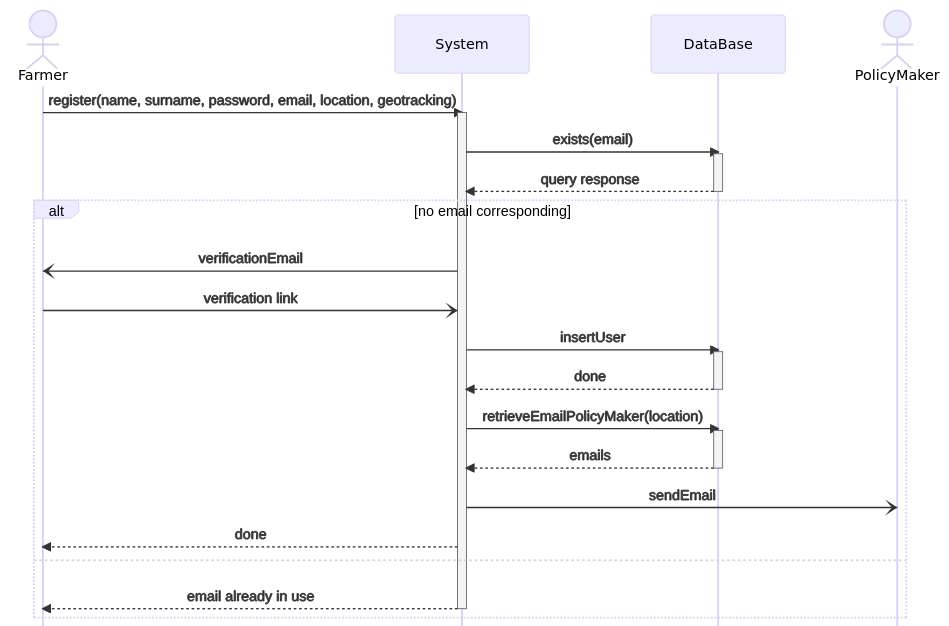
\includegraphics[width=\textwidth]{Images/seq_registration.png}
	\caption{\label{fig:seq_registration} Registration of a Farmer}
\end{figure}

\begin{figure} [H]
	\centering
	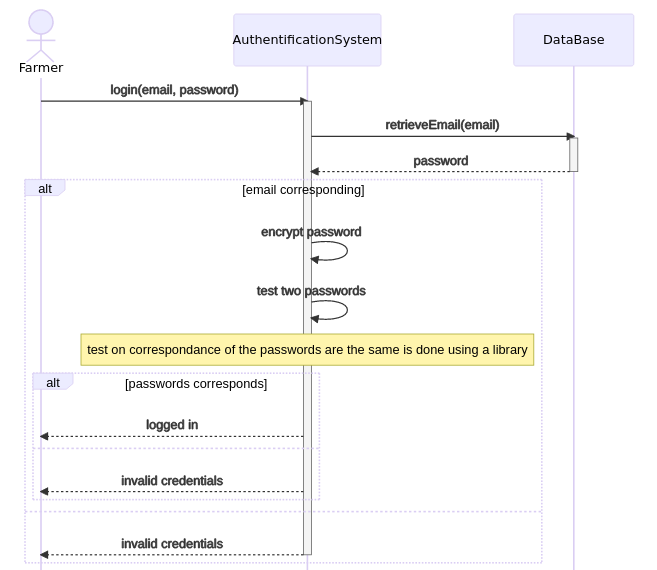
\includegraphics[width=\textwidth]{Images/seq_login.png}
	\caption{\label{fig:seq_login} Login of a Farmer}
\end{figure}

\begin{figure} [H]
	\centering
	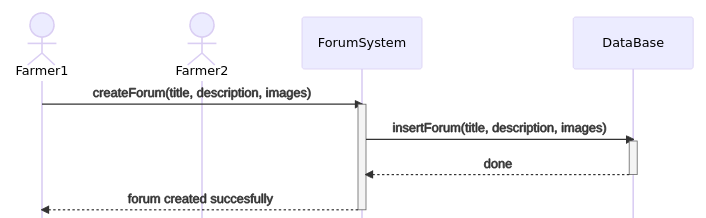
\includegraphics[width=\textwidth]{Images/seq_forum_creation.png}
	\caption{\label{fig:seq_crea_forum} Creation of a forum}
\end{figure}

\begin{figure} [!h]
	\centering
	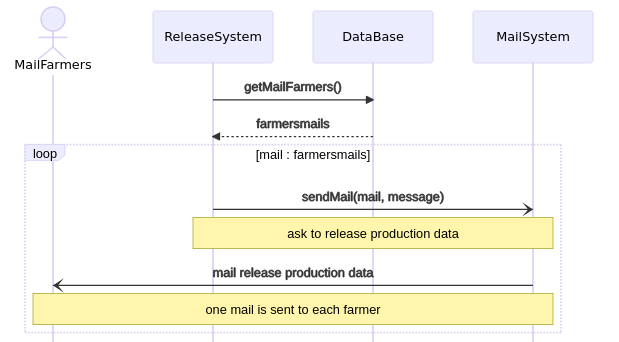
\includegraphics[width=\textwidth]{Images/seq_asking_prod_data.png}
	\caption{\label{fig:seq_asking_proddata} System asking to farmers to put their production data}
\end{figure}

\begin{figure} [H]
	\centering
	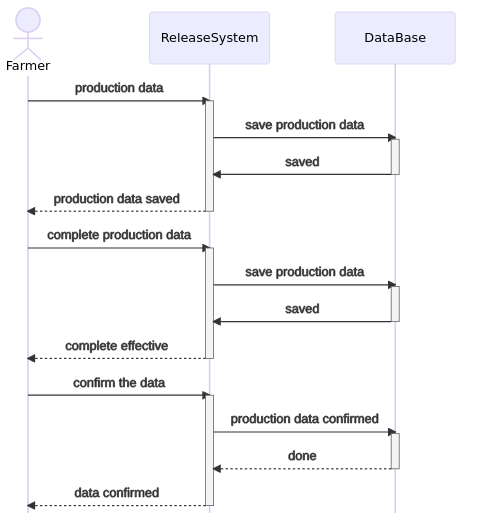
\includegraphics[width=\textwidth]{Images/seq_request_prod_data.png}
	\caption{\label{fig:seq_request_prod_data} Farmer putting their production data}
\end{figure}
\subsection{Component interfaces}
In the following diagram, the DBMS interfaces are not covered since they are supposed to execute basic queries that can be handled by any system.

\begin{figure} [H]
	\centering
	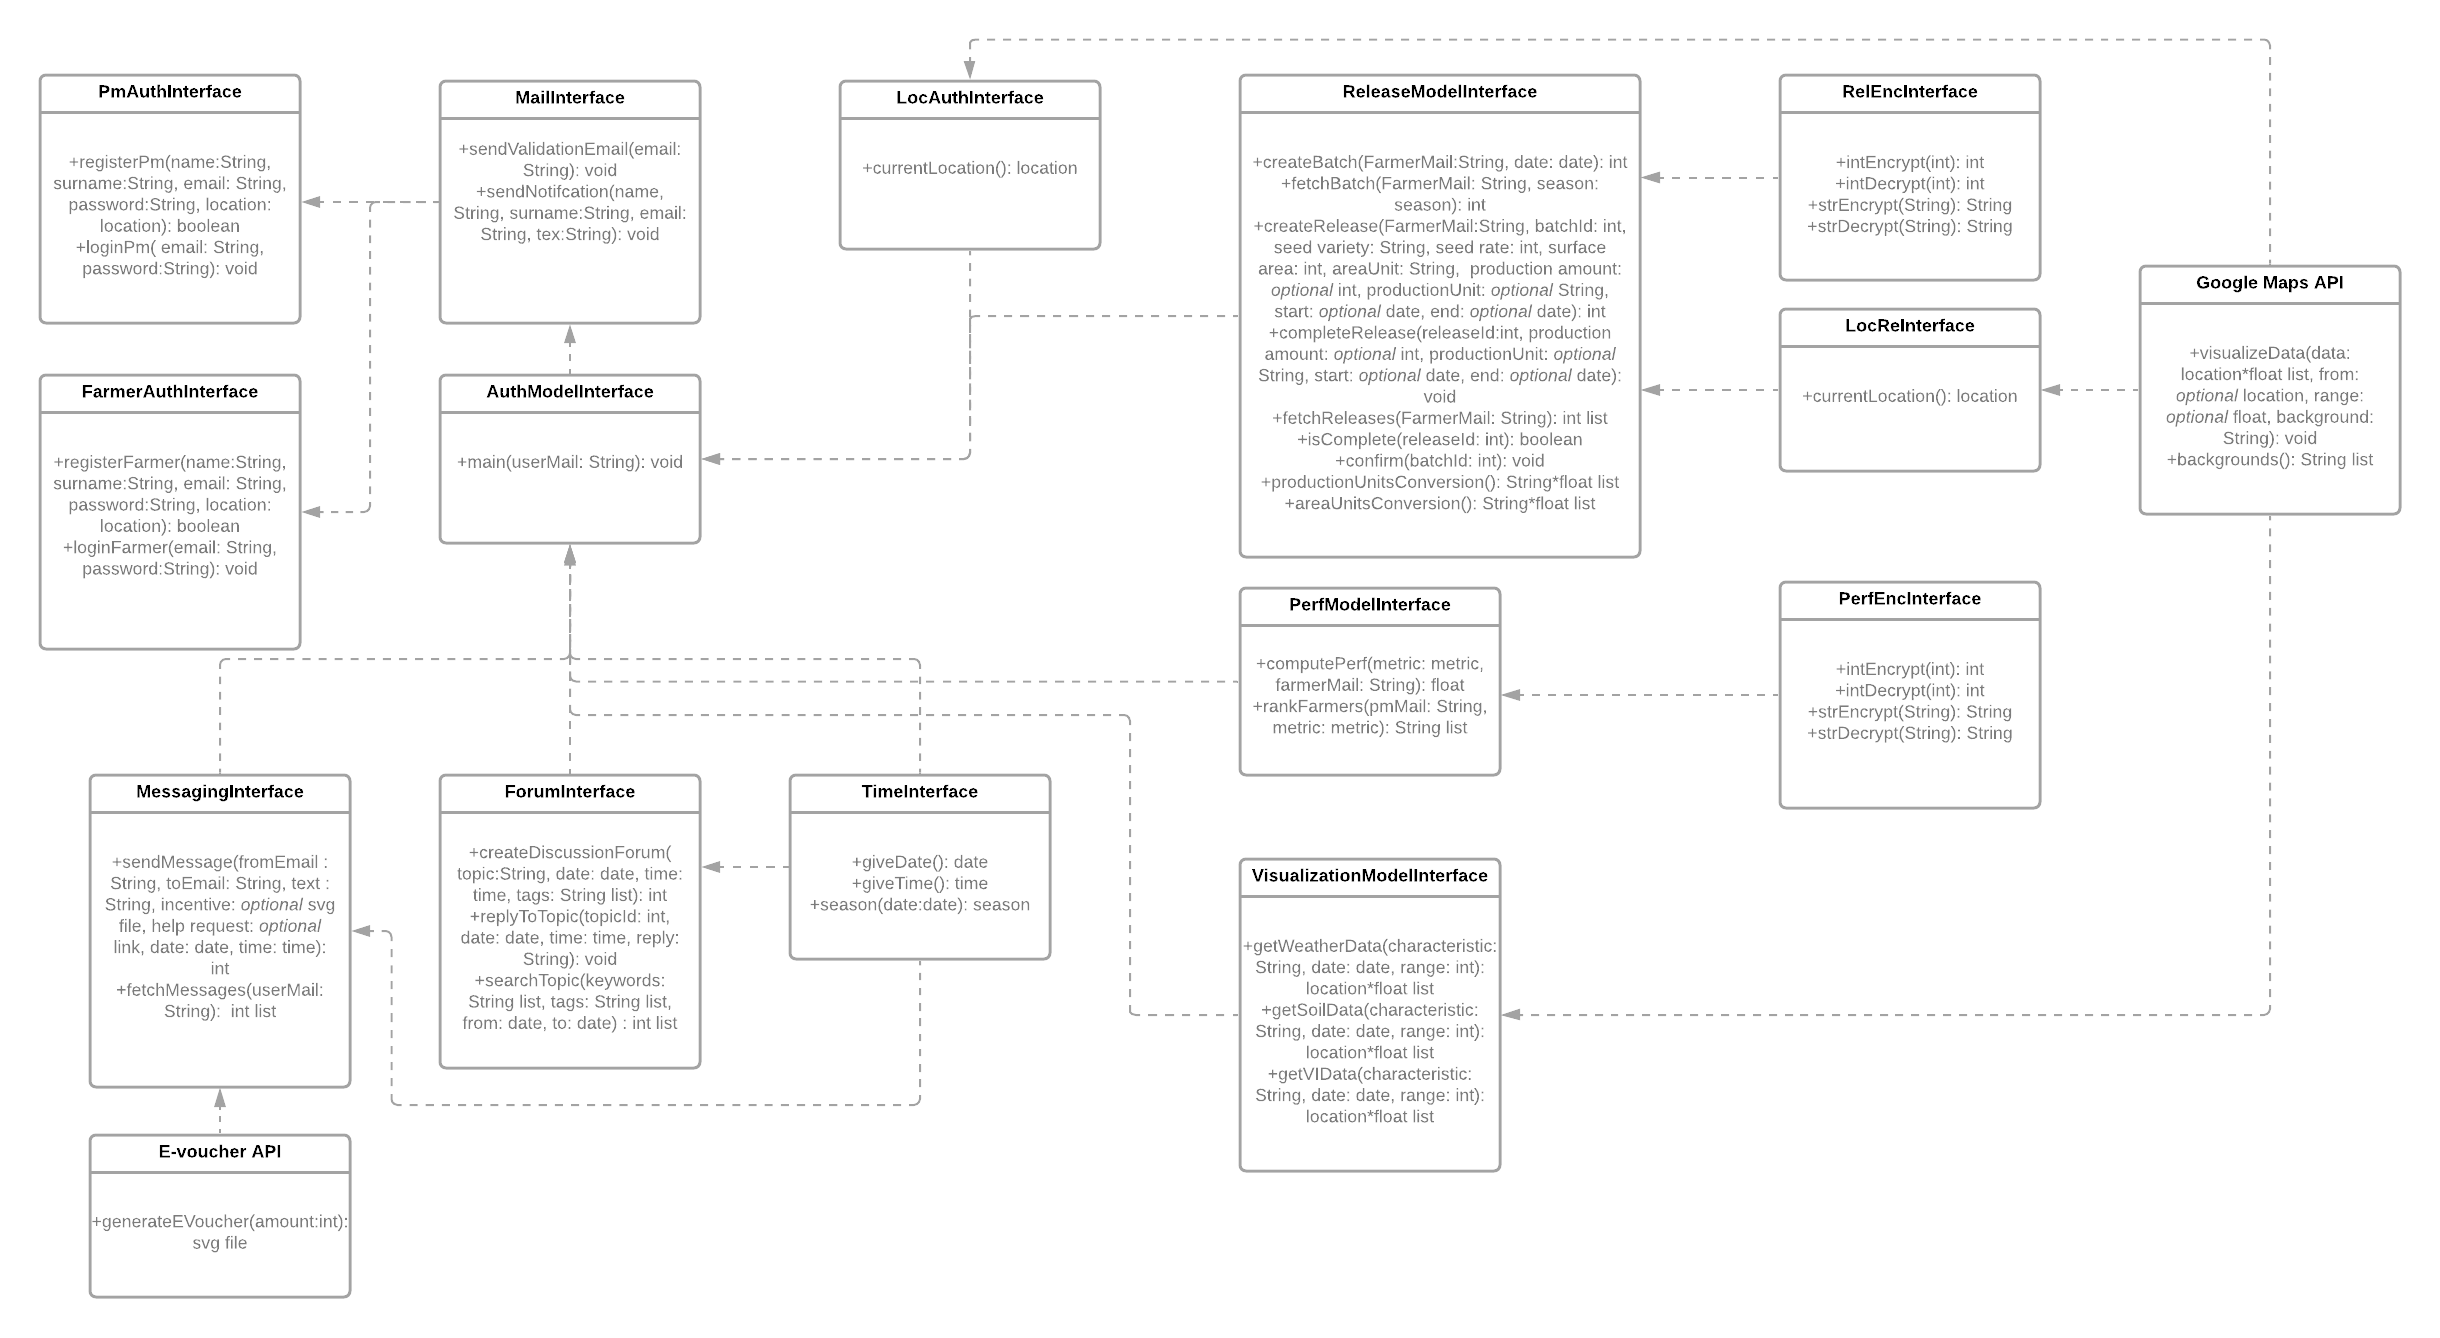
\includegraphics[width=\textwidth]{Images/component-interfaces-diagram.png}
	\caption{\label{fig:component_interfaces_diag} Component interfaces diagram}
\end{figure}

\subsection{Selected architectural styles and patterns}
Since the application is distributed and explicitly designed to support interface between users and the system, the optimal architecture is a client/server one. 

As the system integrates multiple data sources, a three-tier architecture is more adequate. The system is thus divided into a Client Layer, which is the entry point for users, the Business Layer which is embedded in servers, and the Data Layer. 

For the sake of simplicity, praticality and security, the architecture is designed as a thin client one.
